\chapter{Formalization of \bil}

At the core of \bap is the \bap intermediate language, called \bil. In
this chapter we present a formalization of \bil. The formalization is
intended to provide an exact description of what we mean by statements
in the IL.

{\it Note:} In our implementation, as discussed elsewhere, there are
actually several IL's.  Throughout this chapter we discuss the IL as
implemented in {\tt ast.ml}.  The other IL's differ in uninteresting
ways and are variants of the IL discussed here. In particular,
developers will be interested in {\tt ssa.ml}, which defines the IL in
SSA form, and also does not allow recursively defined expressions
(i.e., it is an SSA three-address code).  Thus, this chapter can be
viewed as a specification for the actual code.



\section{The \bil Language}
\label{vine:language}


\begin{table}
\centering
\begin{tabular}{lll}
  \emphkind{program}&::=&
        \emphkind{stmt}*\\

  \emphkind{stmt}&::=&  
         \emphkind{var} := \emphkind{exp}
     $|$ {\tt jmp}(\emphkind{exp})
     $|$ {\tt cjmp}(\emphkind{exp},\emphkind{exp},\emphkind{exp})\\
     &&$|$ {\tt halt}(\emphkind{exp})
     $|$ {\tt assert}(\emphkind{exp})
     $|$ {\tt label} \emphkind{label\_kind}
     $|$ {\tt special}(string)\\

  \emphkind{exp}&::=& 
         {\tt load}(\emphkind{exp}, \emphkind{exp}, \emphkind{exp},
         \emphkind{$\tau_{\text{reg}}$})
        $|$ {\tt store}(\emphkind{exp}, \emphkind{exp},
        \emphkind{exp},\emphkind{exp},$\tau_{\text{reg}}$ )
     $|$ \emphkind{exp} $\Diamond_b$ \emphkind{exp}
     \\
     & & 
     $|$ $\Diamond_u$ \emphkind{exp}
     $|$ \emphkind{var}
     $|$ {\tt lab}(string)
     $|$ \emphkind{integer}
     $|$ {\tt
       cast}(\emphkind{cast\_kind},$\tau_{\text{reg}}$,\emphkind{exp})
\\
     & & $|$ {\tt let} \emphkind{var} {\tt =} \emphkind{exp} {\tt in} \emphkind{exp}
    
     $|$ {\tt unknown}(string, $\tau$)
     $|$ {\tt name}(\emphkind{exp})
     \\

  \emphkind{label\_kind}&::=&  \emphkind{integer} $|$ string \\
     
  \emphkind{cast\_kind}&::=&  
     {\tt unsigned}
     $|$ {\tt signed}
     $|$ {\tt high} 
     $|$ {\tt low}\\

%   \emphkind{decl}&::=& 
%          {\tt var} \emphkind{var}\\


  \emphkind{var}&::=& 
         (string, id$_v$, $\tau$)\\

  $\Diamond_b$&::=&
     $+ , - , * ,  /, /_s , \bmod , \bmod_s , \ll, \gg, \gg_a ,  \&,
        |, \xor, ==, !=, <, \leq , <_s, \leq_s$\\

  $\Diamond_u$&::=& $-$ (unary minus), $\sim$ (bit-wise not)\\

  \emphkind{value}&::=&  \emphkind{integer}
       $|$ \emphkind{memory} 
       $|$ string
       $|$ $\perp$  \\

  \emphkind{integer}&::=&          $n$ (:$\tau_{\text{reg}})$ \\


  \emphkind{memory}&::=&
        \{ \emphkind{integer} $\rightarrow$ \emphkind{integer}, 
             \emphkind{integer} $\rightarrow$ \emphkind{integer},
             \ldots \} (:$\tau_{\text{mem}}$) \\

  \emphkind{$\tau$} &::=&
          \emphkind{$\tau_{\text{reg}}$} 
      $|$ \emphkind{$\tau_{\text{mem}}$}\\

  \emphkind{$\tau_{\text{mem}}$} &::=& {\tt mem\_t}($\tau_{\text{reg}}$)
  $|$ {\tt array\_t}($\tau_{\text{reg}}, \tau_{\text{reg}}$)\\\
  
  \emphkind{$\tau_{\text{ reg}}$}&::=&
         {\tt reg1\_t} 
      $|$ {\tt reg8\_t} 
      $|$ {\tt reg16\_t} 
      $|$ {\tt reg32\_t} 
      $|$ {\tt reg64\_t}\\



\end{tabular}
\caption{The Binary Intermediate Language. Note commas separte
  operators.}
\label{vine:syntax}
\end{table}



Table~\ref{vine:syntax} shows the syntax of \bil. We use the term
``instruction'' to refer to an assembly-level instruction, and the
term ``statement'' to refer to instructions within \bil.  Thus, \bap
raises instructions to statements in \bil.  In %% \ref{vine:typecheck}
%% we give basic type-checking rules which disallow certain syntactically
%% valid but nonsensical expressions, and in
~\ref{vine:operational} we
provide the operational semantics. In the remainder of this section we
give an informal description and motivation for constructs in the IL.


\subsection{Values and Types}
The base types $\tau_{\text{reg}}$ in \bil IL are 1, 8, 16, 32, and
64-bit registers (i.e., $n$-bit vectors), and memories. Memories are
given type ${\tt mem\_t}(\tau_{\text{reg}})$, where $\tau_{\text{reg}}$
determines the type for memory addresses. For example, ${\tt
  mem}(\tau_{\text{reg32\_t}})$ corresponds to memory on a typical
32-bit machine.  

We also have arrays, which are given type ${\tt
  array\_t}(\tau_{\text{reg}},\tau_{\text{reg}})$. The tuple
$(\tau_{\text{reg}},\tau_{\text{reg}})$ specifies the index and
element type of an array, respectively.  As we will see, we use arrays
to \emph{normalize} endianed memory accesses.

There are three types of values in \bil. First, \bil has numbers $n$
of type $\tau_{\text{reg}}$. Second, \bil has memory values $\{
n_{a1} \rightarrow n_{v1}, n_{a2} \rightarrow n_{v2}, ... \}$, where
$n_{ai}$ denotes a number used as an address, and $n_{vi}$ denotes the
value stored at the address.  Finally, \bil has a nonsense value
$\perp$. $\perp$ values are not exposed to the user and cannot be
constructed in the presentation language.  $\perp$ is used internally
to indicate a failed execution.


\subsection{Expressions}
Expressions in \bil are side-effect free, and are similar to those
found in most languages.  \bil has binary operations $\Diamond_b$
(note ``\&'' and ``$|$'' are bit-wise), unary operations $\Diamond_u$,
constants, {\tt let} bindings, and casting.  Casting is used when
indexing registers under different addressing modes. For example, the
lower 8 bits of {\tt eax} in x86 are known as {\tt al}.  When lifting
x86 instructions, we use casting to project out the lower-bits of the
corresponding {\tt eax} register variable to an {\tt al} register
variable when {\tt al} is accessed.

The semantics of ${\tt load}(e_1, e_2, e_3, \tau_{\text{reg}})$ is to
load from the memory specified by $e_1$ at address $e_2$. In C, this
would loosely be written $e_1[e_2]$.  The parameter $e_3$ tells us the
endianness to use when loading bytes from memory. $e_3$ is forced to
be of type bool, where we arbitrary affix the meaning that 0 is little
endian and 1 is big endian (since 0 is ``littler'' than 1). Some
architecture consistently use the same endianness, e.g., for x86, the
value of $e_3$ will always correspond to little-endianness.  However,
other architectures such as ARM specify the endianness of a load at
run-time.  Finally, $\tau_{\text{reg}}$ tells us how many bytes to
load.  In C, if $e_1$ is of type $\tau$, then $e_1[e_2]$ loads {\tt
  sizeof($\tau$)} bytes.  $\tau_{\text{reg}}$ similarly tells us how
many bytes to load from memory. While technically we could infer
$\tau_{\text{reg}}$ given $e_1$, we keep it in the IL explicitly for
efficiency.


In \bil, the {\tt store} operation is pure (i.e., side-effect
free). The advantage of pure memory operations in \bil notation is it
makes it possible to syntactically distinguish what memory is modified
or read.  One place we take advantage of this is in SSA where both
scalars and memory have a unique single static assignment location.

Each {\tt store} expression must specify what memory to load or store
from.  The resulting memory is returned as a value.  The semantics of
${\tt store}(e_1, e_2, e_3, e_4, \tau_{\text{reg}})$ are to store in
memory $e_1$, starting at address $e_2$ the value $e_3$.  The store is
performed given the endianness of $e_4$.  This may seem very
complicated when reading. However, the operational semantics are quite
simple: you may want to read the  {\sc store} rules.


The last expression type of note is {\tt unknown}.  An {\tt unknown}
specifies an operation we could not lift to \bil.  The purpose of an
unknown is to adhere to the \bap principle to \emph{know what you do
  not know}.  Consider the case where Intel adds a new instruction,
e.g., as happens in each processor revision.  \bap may not know about
such instructions, thus cannot raise it to \bil. One option would be
to ignore such instructions. However, the result of any analysis would
be suspect in this case. A sound option is to abort lifting and raise
an error. However, we often end up not interested in particular
instructions. Our solution is to raise such instructions, when
possible, to an assignment (where the left hand side is of the correct
type and name) with the actual operation left unspecified as {\tt
  unknown}.

\subsection{Statements and Programs}

A program in \bil is a sequence of statements.  There are 7 different
kinds of instructions. The language has assignments, jumps,
conditional jumps, and labels.  The target of all jumps and
conditional jumps must be a valid label in our operational semantics,
else the program terminates in the error state ($\perp$).  Note that a
jump to an undefined location (e.g., a location that was not
disassembled such as to dynamically generated code) results in the
\bap program halting with $\perp$ (see~\ref{vine:operational}). A
program can halt normally at any time by issuing the {\tt halt}
statement.  We also provide {\tt assert}, which acts similar to a C
assert: the asserted expression must be true, else the machine halts
with $\perp$.

A {\tt special} in \bil corresponds to a call to an externally
defined procedure or function. {\tt special} statements typically
arise from system calls.  The {\tt id} of a {\tt special} indexes the
kind of special, e.g., what system call.

The semantics of {\tt special} are up to the analysis; its operational
semantics are not defined (Chapter~\ref{vine:operational}).  We
include {\tt special} as an instruction type to explicitly distinguish
calls that alter the soundness of an analysis. A typical approach to
dealing with {\tt special} is to replace {\tt special} with an
analysis-specific summary function written in the \bap IL that is
appropriate for the analysis.


\begin{figure}

\subfloat[][]{
\begin{minipage}[b]{2.5in}
\begin{footnotesize}
\begin{tightcode}
// x86 instr dst,src\newline
1. mov [eax], 0xaabbccdd\newline
2. mov ebx, eax\newline
3. add ebx, 0x3\newline
4. mov eax, 0x1122\newline
5. mov [ebx], ax\newline
6. sub ebx, 1\newline
7. mov ax, [ebx]\newline
\end{tightcode}
\end{footnotesize}
\end{minipage}
\label{endian:code}
}
%\begin{minipage}[c]{5in}
%\begin{subfigure}
\subfloat[][]{
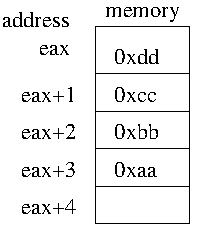
\includegraphics[scale=.7]{fig/memvsarray-1}
\label{endian:membefore}
}
\subfloat[][]{
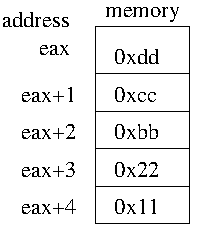
\includegraphics[scale=.7]{fig/memvsarray-2}
\label{endian:memafter}
}
%\end{subfigure}
%\end{minipage}
\caption{(a) shows an example of little-endian stores as found in x86 that
  partially overlap. (b) shows memory after executing line 1, and (c)
  shows memory after executing line 5. Line 7 will load the value 0x22bb.}
\label{fig:endian}
\end{figure}

\section{Normalized Memory} 
\label{vine:normalized}

The endianness of a machine is usually specified by the byte-ordering
of the hardware.  Little endian architectures such as x86 put the
low-order byte first. Big-endian architecture put the high-order byte
first. Some architectures, such as ARM, allow the endianness to be
specified by the instruction, e.g., {\tt mov} would take three
arguments: the source, destination, and endianness for which to
perform the move.


We must take endianness into account when analyzing memory
accesses. Consider the assembly in Figure~\ref{endian:code}. The {\tt
  mov} operation on line 2 writes 4 bytes to memory in little endian
order (since x86 is little endian). After executing line 2, the
address given by {\tt eax} contains byte {\tt 0xdd}, {\tt eax+1}
contains byte {\tt 0xcc}, and so on, as shown in
Figure~\ref{endian:membefore}. Lines 2 and 3 set {\tt ebx =
  eax+2}. Line 4 and 5 write the 16-bit value {\tt 0x1122} to {\tt
  ebx}.  An analysis of these few lines of code needs to consider that
the write on line 4 overwrites the last byte written on line 1, as
shown in Figure~\ref{endian:memafter}. Considering such cases requires
additional logic in each analysis. For example, the value loaded on
line 7 will contain one byte from each of the two stores.

%  In normalized memory,
% all addresses are of the same type $\tau_{\text{addr}} \in
% \tau_{\text{reg}}$, and all values are of type {\tt reg8\_t}.

\begin{figure}
\begin{footnotesize}
\begin{code}  
1. mem4 = let mem1 = store(mem0,eax, 0xdd, 0, reg8\_t) in 
           let mem2 = store(mem1, eax+1, 0xcc, 0, reg8\_t) in 
           let mem3 = store(mem2, eax+2, 0xbb, 0, reg8\_t) in 
               store(mem3, eax+3, 0xcc, 0, reg8\_t);
...
5. mem6 = let mem5 = store(mem4, ebx, 0x22, 0, reg8\_t) in 
             store(mem5, ebx+1, 0x22, 0, reg8\_t) 
...
7. value = let b1 = load(mem6, ebx, 0, reg8\_t) in
            let b2 = load(mem6, ebx+1, 0, reg8\_t) in 
            let b1' = cast(unsigned, b1, 0, reg16\_t) in 
            let b2' = cast(unsigned, b2, 0, reg16\_t) in 
               (b2' $\ll$ 8) $|$ b1';
\end{code}
\end{footnotesize}
\caption{Normalized version of the store and load from Figure~\ref{endian:code}.}
\label{endian:normalized}
\end{figure}


We say a memory is \emph{normalized} for a $b$-byte addressable memory
if all loads and stores are exactly $b$-bytes and $b$-byte
aligned. In x86, memory is byte addressable, so a
normalized memory for x86 has all loads and stores at the byte
level. The normalized form for the write on Line 1 of
Figure~\ref{endian:code} in \bil is shown in
Figure~\ref{endian:normalized}.  Note that the subsequent load on line 7
is with respect to the current memory {\tt mem6}.

Normalized memory makes writing program analyses involving memory
easier.  Analysis is easier because normalized memory syntactically
exposes memory updates that are otherwise implicitly defined by the
endianness.  As a result, analyses do not have to reason explicitly
about overlapping memory, byte order, etc. \bap provides utilities for
normalizing all memory operations so that users can write analysis
more easily.



% Endianness can complicate analysis. 
% specified bit-ordering of the hardware, i.e., a specification of which
% hardware bit corresponds to the low-order bit in a number. 

% Assembly memory operations are
% performed with respect to the endianness (byte ordering) of the
% hardware. 

% A memory operation may either be little endian or big
% endian. A little endian operation to address $a$ stores the low-order
% byte in a register in the lowest memory address, the next lowest-order
% byte in the



% We provide routines to conver little and big endian memories to
% normalized form. The advantage of normalized memory is it eases
% analysis.  For example, consider the x86 instruction sequence shown
% in Figure~\ref{fig:memvsarray}.

% Instruction 1 stores the value 0xaabbccdd into the address given by
% {\tt \%eax}. Since x86 is little-endian, the bytes are stored in
% memory from lowest to highest, as shown in Figure~\ref{fig:}.

% which stores the value in the 4-byte {\tt \%ebx} register
% into the address given by {\tt \%eax}. This instruction on x86 is
% syntatic sugar for storing the low-order byte of {\tt \%ebx} at
% address {\tt \%eax}, the second low-order byte in {\tt \%eax+1}, the
% third in {\tt \%eax+2}, and the high-order byte in {\tt \%eax+3}. In
% \bap, a normalized memory desugars such statements, so {\tt mov
%   *\%eax, \%ebx} becomes:
% \begin{footnotesize}
% \begin{code}
%   // mov *\%eax, \%ebx is desugared in normalized vine memory as
%     mem1 = store(mem0, eax,   ebx \& 0x000000ff);
%     mem2 = store(mem1, eax+1, ebx \& 0x0000ff00);
%     mem3 = store(mem2, eax+2, ebx \& 0x00ff0000);
%     mem4 = store(mem3, eax+3, ebx \& 0xff000000);
% \end{code}
% \end{footnotesize}


% Typically an assembly program works on a single memory.  

% Values in \bap are either register values or memories.  

% Scalar variables in \bap roughly correspond to registers. Although

% In this section we describe the \bap IL.  We first present the \bap
% IL.  In \bap, we have several statements that are derived
% forms. These derived forms are a ``syntatic sugar'' that make writing
% analysis easier, though add no real power to the language.  As
% mentioned, one of the principles of \bap is to treat assembly as a
% first class language. One consequence is \bap does not have
% functions. However, we have observed that several analysis benefit
% from assuming functions exist. We present \bap$_f$, which is an
% extension to \bap which includes functions.



% subsection

%\subsection{\bap and the Running Example}

\begin{figure}
\begin{minipage}[c]{.45\linewidth}
  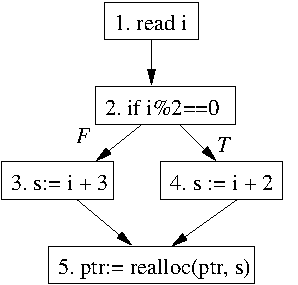
\includegraphics{fig/running-example}
  \label{vine:running-example-fig}
\end{minipage}
\begin{scriptsize}
\begin{minipage}[c]{.45\linewidth}
\begin{lstlisting}
// address instr dst, src
0x8048419 push   ebp  // setup stack
0x804841a mov    ebp,esp
0x804841c sub    esp, 0x18
0x804841f lea    eax, [ebp-0x8]
0x8048422 mov    [esp], eax 
0x8048425 call   0x80483f4 // call read
0x804842a mov    eax, [ebp-0x8]
0x804842d and    eax, 0x1  // if i%2==0
0x8048430 test   eax,eax
0x8048432 jne    0x804843f
0x8048434 mov    eax,[ebp-0x8]
0x8048437 add    eax, 0x2  // s := i+2
0x804843a mov    [ebp-0x4], eax
0x804843d jmp    0x8048448
0x804843f mov    eax,[ebp-0x8]
0x8048442 add    eax,0x3  // s := i+3
0x8048445 mov    [ebp-0x4], eax
0x8048448 mov    eax, [ebp-0x4]
0x804844b mov    [esp+0x4], eax
0x804844f mov    eax, [ebp+0x8]
0x8048452 mov    [esp],eax
0x8048455 call   0x8048338 // call realloc
0x804845a mov    [ebp+0x8],eax
0x804845d leave  
0x804845e ret    
\end{lstlisting}
\end{minipage}
\end{scriptsize}
\caption{Our running example from \ref{intro:running} on the  left, and the
  corresponding x86 assembly in Intel syntax on the right.}
\label{fig:running-asm}
\end{figure}

% \begin{figure}
% \begin{scriptsize}
% \begin{minipage}[c]{.45\linewidth}
% \begin{lstlisting}
% 0x8048419 push   ebp
% 0x804841a mov    ebp,esp
% 0x804841c sub    esp, 0x18
% 0x804841f lea    eax, [ebp-0x8]
% 0x8048422 mov    [esp], eax
% 0x8048425 call   0x80483f4
% 0x804842a mov    eax, [ebp-0x8]
% 0x804842d and    eax, 0x1
% 0x8048430 test   eax,eax
% 0x8048432 jne    0x804843f
% 0x8048434 mov    eax,[ebp-0x8]
% 0x8048437 add    eax, 0x2
% \end{lstlisting}
% \end{minipage}
% \begin{minipage}[c]{.45\linewidth}
% \begin{lstlisting}
% 0x804843a mov    [ebp-0x4], eax
% 0x804843d jmp    0x8048448
% 0x804843f mov    eax,[ebp-0x8]
% 0x8048442 add    eax,0x3
% 0x8048445 mov    [ebp-0x4], eax
% 0x8048448 mov    eax, [ebp-0x4]
% 0x804844b mov    [esp+0x4], eax
% 0x804844f mov    eax, [ebp+0x8]
% 0x8048452 mov    [esp],eax
% 0x8048455 call   0x8048338
% 0x804845a mov    [ebp+0x8],eax
% 0x804845d leave  
% 0x804845e ret    
% \end{lstlisting}
% \end{minipage}
% \end{scriptsize}
% \caption{The running example from Figure~\ref{vine:running-example-fig} in
%   Intel-syntax x86 assembly.}
% \label{fig:running-asm}
% \end{figure}


%\begin{figure}
\begin{scriptsize}
\begin{minipage}[c]{.50\linewidth}
\begin{lstlisting}
label 0x8048419; //push   ebp
  ESP = ESP - 4;
  mem = store(mem, ESP, EBP, reg32_t);
label 0x804841a; //mov    ebp,esp
  EBP = ESP;
label 0x804841c; //sub esp, 0x18
  ESP = ESP-24; 
  /* 'sub' eflags omitted */
label 0x804841f; //lea    eax, [ebp-0x8]
  EAX = (EBP+0xFFFFFFF8);
label 0x8048422; //mov    [esp], eax
  mem = store(mem, ESP, EAX, reg32_t);
label 0x8048425; //call   0x80483f4
  ESP = ESP-4;
  mem = store(mem, ESP, 0x804842A, reg32_t);
  jmp(0x80483f4); 
label 0x804842a; //mov    eax, [ebp-0x8]
  EAX = load(mem, EBP+0xFFFFFFF8,reg32_t);
label 0x804842d; //and    eax, 0x1
  EAX = EAX & 1; 
  /* 'and' eflags omitted */
label 0x8048430; //test   eax,eax
  temp = EAX & EAX;
  ZF:reg1_t = temp == 0; 
  /* SF and PF code omitted */
label 0x8048432; //jne    0x804843f
  cjmp(ZF,0x8048434,0x804843F);
label 0x8048434; //mov    eax,[ebp-0x8]
  EAX = load(mem, EBP+0xFFFFFFF8, reg32_t);
label 0x8048437; //add    eax, 0x2 
  EAX = EAX + 2; 
  /* 'add' eflags omitted */
\end{lstlisting}
\end{minipage}
\begin{minipage}[c]{.45\linewidth}
\begin{lstlisting}
label 0x804843a; //mov    [ebp-0x4], eax
  mem = store(mem, EBP+0xFFFFFFFC, EAX, reg32_t);
label 0x804843d; //jmp    0x8048448
  jmp(0x8048448);
label 0x804843f; //mov    eax,[ebp-0x8]
  EAX = load(mem, EBP+0xFFFFFFF8, reg32_t);
label 0x8048442; //add    eax,0x3
  EAX = EAX+3; 
  /* 'add' eflags omitted */
label 0x8048445; //mov    [ebp-0x4], eax
  mem = store(mem, EBP+0xFFFFFFFC, EAX, reg32_t);
label 0x8048448; //mov    eax, [ebp-0x4]
  EAX = load(mem, EBP+0xFFFFFFFC, reg32_t);
label 0x804844b; //mov    [esp+0x4], eax
  mem = store(mem, ESP+4, EAX, reg32_t);
label 0x804844f; //mov    eax, [ebp+0x8]
  EAX = load(mem, EBP+8, reg32_t);
label 0x8048452; //mov    [esp],eax
  mem = store(mem, ESP, EAX, reg32_t);
label 0x8048455; //call   0x8048338
  ESP = ESP-4;
  mem = store(mem, ESP, 0x804845A, reg32_t);
  jmp(0x8048338); 
label 0x804845a; //mov    [ebp+0x8],eax
  mem = store(mem, ESP+8, EAX, reg32_t);
label 0x804845d; //leave
  ESP = EBP+4;
  EBP = load(mem, EBP, reg32_t);
label 0x804845e; //ret
  target = load(mem, ESP, reg32_t);
  ESP = ESP+4;
  jmp(target);
\end{lstlisting}
\end{minipage}
\end{scriptsize}
\caption{The assembly from Figure~\ref{fig:running-asm} in the \bap IL.}
\label{fig:running-il}
\end{figure}

Figure~\ref{fig:running-asm} shows the assembly for the running
example from \chref~1 (which is reproduced as part of the figure). The
assembly (given in Intel syntax) shown is for the running example
compiled as a single function which is passed in {\tt ptr}, with {\tt
read} and {\tt realloc} as external calls.  Each assembly line
contains the instruction address followed by the instruction with
operands.

The first 4 instructions in Figure~\ref{fig:running-asm} implement the
function prologue, which sets up the stack frame.  The variable {\tt i}
is assigned by the compiler to register {\tt eax}. Instruction
0x804822-0x804825 push the argument {\tt eax} onto the stack, and then
call the function corresponding to {\tt read} at address 0x80483f4.
Instruction 0x804842d-0x8048430 correspond to the test {\tt if i \%2
== 0}.  The compiler implemented the reduction modulo 2 as bit-wise ``and''.
Instructions 0x8048437-0x804843d implement the true branch where {\tt
s := i+2}.  The compiler assigned the variable {\tt s} the register
{\tt eax} in assembly, which is put on the local stack frame slot {\tt
ebp-0x4}.  Instructions 0x8048442-0x8048445 implement the false branch
where {\tt s := i+3}, again storing the result in {\tt ebp-0x4}.  Line
0x804844b-0x48455 correspond to the call to {\tt realloc}, followed by
the function epilogue.

\begin{figure}
\begin{scriptsize}
\begin{minipage}[c]{.50\linewidth}
\begin{lstlisting}
label 0x8048419; //push   ebp
  ESP = ESP - 4;
  mem = store(mem, ESP, EBP, reg32_t);
label 0x804841a; //mov    ebp,esp
  EBP = ESP;
label 0x804841c; //sub esp, 0x18
  ESP = ESP-24; 
  /* 'sub' eflags omitted */
label 0x804841f; //lea    eax, [ebp-0x8]
  EAX = (EBP+0xFFFFFFF8);
label 0x8048422; //mov    [esp], eax
  mem = store(mem, ESP, EAX, reg32_t);
label 0x8048425; //call   0x80483f4
  ESP = ESP-4;
  mem = store(mem, ESP, 0x804842A, reg32_t);
  jmp(0x80483f4); 
label 0x804842a; //mov    eax, [ebp-0x8]
  EAX = load(mem, EBP+0xFFFFFFF8,reg32_t);
label 0x804842d; //and    eax, 0x1
  EAX = EAX & 1; 
  /* 'and' eflags omitted */
label 0x8048430; //test   eax,eax
  temp = EAX & EAX;
  ZF:reg1_t = temp == 0; 
  /* SF and PF code omitted */
label 0x8048432; //jne    0x804843f
  cjmp(ZF,0x8048434,0x804843F);
label 0x8048434; //mov    eax,[ebp-0x8]
  EAX = load(mem, EBP+0xFFFFFFF8, reg32_t);
label 0x8048437; //add    eax, 0x2 
  EAX = EAX + 2; 
  /* 'add' eflags omitted */
\end{lstlisting}
\end{minipage}
\begin{minipage}[c]{.45\linewidth}
\begin{lstlisting}
label 0x804843a; //mov    [ebp-0x4], eax
  mem = store(mem, EBP+0xFFFFFFFC, EAX, reg32_t);
label 0x804843d; //jmp    0x8048448
  jmp(0x8048448);
label 0x804843f; //mov    eax,[ebp-0x8]
  EAX = load(mem, EBP+0xFFFFFFF8, reg32_t);
label 0x8048442; //add    eax,0x3
  EAX = EAX+3; 
  /* 'add' eflags omitted */
label 0x8048445; //mov    [ebp-0x4], eax
  mem = store(mem, EBP+0xFFFFFFFC, EAX, reg32_t);
label 0x8048448; //mov    eax, [ebp-0x4]
  EAX = load(mem, EBP+0xFFFFFFFC, reg32_t);
label 0x804844b; //mov    [esp+0x4], eax
  mem = store(mem, ESP+4, EAX, reg32_t);
label 0x804844f; //mov    eax, [ebp+0x8]
  EAX = load(mem, EBP+8, reg32_t);
label 0x8048452; //mov    [esp],eax
  mem = store(mem, ESP, EAX, reg32_t);
label 0x8048455; //call   0x8048338
  ESP = ESP-4;
  mem = store(mem, ESP, 0x804845A, reg32_t);
  jmp(0x8048338); 
label 0x804845a; //mov    [ebp+0x8],eax
  mem = store(mem, ESP+8, EAX, reg32_t);
label 0x804845d; //leave
  ESP = EBP+4;
  EBP = load(mem, EBP, reg32_t);
label 0x804845e; //ret
  target = load(mem, ESP, reg32_t);
  ESP = ESP+4;
  jmp(target);
\end{lstlisting}
\end{minipage}
\end{scriptsize}
\caption{The assembly from Figure~\ref{fig:running-asm} in the \bap IL.}
\label{fig:running-il}
\end{figure}

Figure~\ref{fig:running-il} shows the \bap IL for the assembly in
Figure~\ref{fig:running-asm}. For simplicity, we note where {\tt
eflags} code is calculated, but do not include the logic in the
Figure. Each assembly instruction is lifted in a syntax-directed
manner.

The IL reduces complex x86 instructions to a simplified language. For
example, the x86 {\tt push ebp} instruction at 0x8048419 in the IL is
de-sugared as decrementing the register {\tt esp} by one word, then
storing {\tt ebp} at the resulting address in memory.  Another example
is in assembly, there is no syntactic relationship between the {\tt
test} instruction at 0x8048430 and the conditional jump {\tt jne} at
0x804843f. The IL, however, explicitly shows {\tt test} sets the {\tt
 ZF} flag, which the raised conditional jump checks.



% subsection
%\input{derived}
% subsection
%\subsection{\bap Typing}
\label{vinesec:typecheck}

%\renewcommand{\baselinestretch}{1.0}\normalsize

\begin{table}

{\bf Context}\\
\begin{tabular}{llp{4.5in}}
$\Gamma$ & \emphkind{var} $\rightarrow$ $\tau$& 
Typing context of $(x:\tau)$ pairs where $x$ is of type $\tau$.
\end{tabular}\\[10pt]
{\bf Program and Instructions}
\begin{footnotesize}
\[
\begin{array}{c}
\infer[]
 { 
   \cdot \vdash (x_i:\tau_i)^* i^*  : ()
 }
 {
   \forall i \in i^* | (x_i:\tau_i)^* \vdash i : ()
 }
\end{array}
\]
\[
\begin{array}{ccc}
\infer[\textsc{assign}]
   {
     \Gamma \vdash x := e : ()
   }
   {
     \Gamma \vdash e : \tau
     &
     \Gamma \vdash x : \tau
   } &
\infer[\textsc{jmp}]
   {
     \Gamma \vdash \texttt{jmp($e$)} : ()
   }
   {
     \Gamma \vdash e : \texttt{reg64\_t}
   } & 
\infer[\textsc{halt}]
  {
     \Gamma \vdash \texttt{halt($e$)} : ()
  }
  { 
     \Gamma \vdash e : \tau
     & \tau \in \tau_{\text{reg}}
  }
\end{array}
\]
\[
\begin{array}{c}
\infer[\textsc{cjmp}]
   {
     \Gamma \vdash \texttt{cjmp($e_1$, $e_2$, $e_3$)} : ()
   }
   {
      \Gamma \vdash e_1 : \texttt{reg1\_t}
      & 
      \Gamma \vdash e_2 : \texttt{reg64\_t}
      &
      \Gamma \vdash e_3 : \texttt{reg64\_t}
   }
\end{array}
\]
\[
\begin{array}{ccc}
\infer[\textsc{assert}]
  {
    \Gamma \vdash \texttt{assert($e$)} : ()
  }
  {
    \Gamma \vdash e : \texttt{reg1\_t}
  } &
 \infer[\textsc{label}]
  {
    \Gamma \vdash \texttt{label $n$} : ()
  }
  {
  } &
\infer[\textsc{special}]
  {
   \Gamma \vdash \texttt{special {\sf id$_s$}} : ()
  }
  {
  }
\end{array}
\]
\end{footnotesize}
{\bf Auxiliary Definitions}
\begin{footnotesize}
\[
\begin{array}{c}
 \infer[\textsc{reg-subtype}]
   {
     \texttt{reg1\_t $<:$ reg8\_t $<:$ reg16\_t $<:$ reg32\_t $<:$ reg64\_t}
   }
   {
   }
\end{array}
\]
\[
\begin{array}{cc}
\infer[]
  {
    \text{mem\_compat($\tau_1$, $\tau_2$)}
  }
  {
   \tau_1 = \texttt{big $|$ little} 
    & \tau_2 \in \tau_{\text{reg}} 
  } &
\infer[]
  {
    \text{mem\_compat({\tt norm}, {\tt reg8\_t})}
  }
  {
  }\\[10pt]
\infer[]
  {
    \text{cast\_compat(k, $\tau_1$, $\tau_2$)}
  }
  {
    k = \texttt{unsigned $|$ signed}
    & 
    \tau_1 <: \tau_2
  }&
\infer[]
  {
    \text{cast\_compat(k, $\tau_1$, $\tau_2$)}
  }
  {
    k = \texttt{hi $|$ low}
    & 
    \tau_2 <: \tau_1
  }
\end{array}
\]
\end{footnotesize}
{\bf Expressions}
\begin{footnotesize}
\[
\begin{array}{cc}
\infer[\textsc{load}]
  { % conclusion
    \Gamma \vdash \texttt{load($e_1$, $e_2$, $\tau$)} : \tau
  }
  { % premise
    \Gamma \vdash e_1 : \texttt{mem\_t($\tau_1$, $\tau_2$)}
    & 
    \text{mem\_compat($\tau_1$, $\tau$)}
    &
    \Gamma \vdash e_2 : \tau_2
  } &
\infer[\textsc{var}]
  { % conclusion
      \Gamma \vdash x : \tau
  }
  { % premise
        x:\tau \in \Gamma
  }
\end{array}
\]
\[
\begin{array}{c}
\infer[\textsc{store}]
  { % conclusion
    \Gamma \vdash \texttt{store($e_1$, $e_2$,$e_3$)}:\texttt{mem\_t($\tau_1$, $\tau_2$)}
  }
  { %premise
    \Gamma \vdash e_1: \texttt{mem\_t($\tau_1$, $\tau_2$)}
    &
    \Gamma \vdash e_2 : \tau_2 
    & 
    \Gamma \vdash e_3 : \tau_4
    & 
    \text{mem\_compat($\tau_1$, $\tau_4$)}
  }\\
\end{array}
\]
\[
\begin{array}{cc}
\infer[\textsc{binop$_1$}]
  { % conclusion
    \Gamma \vdash e_1 \Diamond_b e_2 : \tau
  }
  { % premise
    \Gamma \vdash e_1 : \tau 
    & \Gamma \vdash e_2 : \tau
    & \tau \in \tau_{\text{reg}}
    & \Diamond_b \notin \ll, \gg, \gg_a
  } &
\infer[\textsc{unop}]
  { % conclusion
    \Gamma \vdash \Diamond_u e : \tau
  }
  { % premise
    \Gamma \vdash e : \tau 
    & \tau \in \tau_{\text{reg}}
  } 
\end{array}
\]
\[
\begin{array}{c}
\infer[\textsc{binop$_2$}]
  { % conclusion
    \Gamma \vdash e_1 \Diamond_b e_2 : \tau
  }
  { % premise
    \Gamma \vdash e_1 : \tau 
    & \Gamma \vdash e_2 : \tau_2
    & \tau, \tau_2 \in \tau_{\text{reg}}
    & \Diamond_b \in \ll, \gg, \gg_a
  } 
\end{array}
\]
\[
\begin{array}{cc}
\infer[\textsc{cast}]
  { % conclusion 
   \Gamma \vdash \texttt{cast(\emphkind{cast\_kind}, $\tau$, $e$)} : \tau
  }
  { % premise
    \Gamma \vdash e : \tau_1
    & \tau, \tau_1 \in \tau_{\text{reg}}
    & \text{cast\_compat(\emphkind{cast\_kind}, $\tau_1$, $\tau$)}
  } &
\infer[\textsc{let}]
  { % conclusion
    \Gamma \vdash \texttt{let $x$ := $e_1$ in $e_2$} : \tau
  }
  { % premise
    \Gamma \vdash e_1 : \tau_1
    & \Gamma,(x:\tau_1) \vdash e_2 : \tau
  } 

\end{array}
\]
\end{footnotesize}
\caption{Type-checking rules for \bap.}
\label{vine:typecheck}
\end{table}
%\renewcommand{\baselinestretch}{1.66}\normalsize


The \bap IL syntax described in Table~\ref{vine:syntax} is designed
to be simple. A literal interpretation, however, allows several
nonsensical operations such as left-shifting two memory variables.  We
type-check \bap programs using the  rules shown in
Table~\ref{vine:typecheck} to weed out obviously nonsensical
operations.  We emphasize that type-checking to show program safety is outside
the scope of \bap.

The type-checking rules are straight-forward.  \bap requires that
binary and unary operations be on scalars of the same register type
(except shifts where the shift amount need only be an integer). We
type-check {\tt hi} and {\tt low} casts such that the resulting type
is a smaller register type (in terms of the sub-typing relationship
{\sc reg-subtype}), as expected.  {\tt unsigned} and {\tt signed}
casts must be to a wider register type. One issue with un-normalized
memory is that it may have multi-byte accesses, e.g., a store on x86
could be of 32, 16, or 8 bits. Normalized memory, on the other hand,
only allows stores and loads of bytes.  We define an auxiliary
predicate ``mem\_compat'' to ensure that normalized memory is accessed
appropriately.  Also note that as a convenience we assume 64-bit
addressing in the rules, but allow smaller addressable memories via
the {\tt reg-subtype} sub-typing rule.

A program type-checks if all instructions type-check under the
declared variable types.  We require all variables be declared because
explicitly typed languages are easier to check. 


% subsection
\subsection{Operational Semantics}
\label{vine:operational}


%\renewcommand{\baselinestretch}{1.0}\normalsize

\begin{table}
{\bf Contexts}\\
\begin{tabular}{lllp{4in}}
  {\it Instruction} & $\Pi$ & $n$ $\mapsto$ \emphkind{instr} &
  Maps an instruction address to an instruction.\\
  {\it Variable} & $\Delta$ &  $id \mapsto \emphkind{var}$  &Maps
  a variable ID to its value.\\
  {\it Labels} & $\Lambda$ & $\emphkind{label\_kind} \mapsto n$ & Maps
  a label to the address of the corresponding {\tt label} instruction number.
\end{tabular}\\
\newline
{\bf Notation}\\
\begin{tabular}{lp{4.2in}}
  $\Delta \vdash e \Downarrow v$ & Expression $e$ evaluates to value
  $v$ given variable context $\Delta$ as given by the expression
  evaluation rules.\\
  $\Delta' = \Delta[x \leftarrow v]$ & $\Delta'$ is the same as
  $\Delta$ except extended to map $x$  to $v$.\\
  $\Pi \vdash p:i$ & $\Pi$ maps instruction address $p$ to instruction
  $i$. If $p \notin \Pi$, the machine gets stuck.\\
  $\Lambda \vdash v:p$ & $\Lambda$ maps instruction label $v$ to instruction
  address $p$. If $v \notin \Lambda$, then machine gets stuck. In
  addition, a well-formed machine should have $\Pi \vdash p : i$
  where $i = \texttt{label $v$}$, otherwise the machine is stuck.\\
%   $(\Pi, \Delta, p, \iota)$ & An abstract machine configuration.
%   $\Pi$ and $\Delta$ are contexts define above, $p$ is the program
%   counter, and $\iota$ is the current instruction.\\  
  $(\Delta, p, i) \leadsto (\Delta', p', i')$ &  An
  execution step. $p$ and $p'$ are
  the pre and post step program counters, $i$ and $i'$ are the pre and
  post step  instructions, and $\Delta$ and $\Delta'$ are the pre and post
  step variable contexts. Note $\Lambda$ and $\Pi$ are currently static, thus
  for brevity not included in the execution context.\\
\end{tabular}
\caption{Operational semantics notation.}
\end{table}
\begin{table}
{\bf Instructions}
\begin{small}
\[
\begin{array}{cc}
  \infer[\textsc{Assign}]
    { % conclusion
      \Delta, p, \text{x := $e$} 
      \leadsto 
      \Delta', p+1, i
    }
    { % premise
      \Delta \vdash e \Downarrow v 
      & \Delta' = \Delta[x \leftarrow v]
      & \Pi \vdash p+1:i
    } &
  \infer[\textsc{Jmp}]
  { % conclusion
    \Delta, p, \texttt{jmp($\ell$)} 
    \leadsto 
    \Delta, p', \texttt{label $v$}
  }
  { % premise
    \Delta \vdash \ell \Downarrow v
    & \Lambda \vdash v : p'
    & \Pi \vdash p' : \texttt{label $v$}
  }\\[10pt]
  \infer[\textsc{label}]
  { % conclusion
    \Delta, p, \texttt{label $\ell$} 
    \leadsto
    \Delta, p+1, i
  }
  { % premise
      \Pi[p+1] = i
  } &
  \infer[\textsc{halt}]
  { % conclusion
    \Delta, p, \texttt{halt $e$} 
    \leadsto
    \text{terminate with  $v$}
%    \Pi, \Delta, p+1, \texttt{halt $v$}
  }
  {
     \Delta \vdash e \Downarrow v
  }\\[10pt]
  \infer[\textsc{assert-t}]
  { % conclusion
    \Delta, p, \texttt{assert}(e)
    \leadsto
    \Delta, p+1, i
  } 
  { % premise
    \Delta \vdash e \Downarrow 1 &
    \Pi[p+1] = i
  } &
  \infer[\textsc{assert-f}]
  { % conclusion
    \Delta, p, \texttt{assert}(e)
    \leadsto
    \text{terminate with  $\perp$}
  }
  { % premise
    \Delta \vdash e \Downarrow 0
  }
\\
\end{array}
\]
\[
\begin{array}{c}
  \infer[\textsc{CJmp-t}]
  { %conclusion
    \Delta, p, \texttt{cjmp($e$, $\ell_T$, $\ell_F$)} 
    \leadsto
    \Delta, p',  \texttt{label $v$}
  }
  { %premise
    \Delta \vdash e \Downarrow 1
    & \Delta \vdash \ell_T \Downarrow v
    & \Lambda \vdash v: p'
    & \Pi \vdash p' :  \texttt{label $v$}
  }\\[10pt]
  \infer[\textsc{CJmp-f}]
  { %conclusion
    \Delta, p, \texttt{cjmp($e$, $\ell_T$, $\ell_F$)} 
    \leadsto
    \Delta, p', \texttt{label $v$}
  }
  { %premise
    \Delta \vdash e \Downarrow 0
    & \Delta \vdash \ell_F \Downarrow v
    & \Lambda \vdash v: p'
    & \Pi \vdash p' : \texttt{label $v$}
  } \\[10pt]
  \text{No rule for {\tt special}, when
    $v \notin \Lambda$, and when  $p \notin \Pi$.}  
\end{array}
\]
\end{small}

{\bf Expressions}\\
\begin{small}
\[
\begin{array}{cc}
  \infer[\textsc{binop}]
  { % conclusion
    \Delta \vdash e_1 \Diamond_b e_2 \Downarrow v
  }
  { % premise
    \Delta \vdash e_1 \Downarrow v_1 
    & \Delta \vdash e_2 \Downarrow v_2
    & v = v_1 \Diamond_b v_2
  } &
  \infer[\textsc{unop}]
  { % conclusion
    \Delta \vdash \Diamond_u e_1 \Downarrow v
  } 
  { % premise
    \Delta \vdash e_1 \Downarrow v_1 
    & v = \Diamond_u v_1
  }\\[10pt]
\end{array}
\]
\[
\begin{array}{ccc}
  \infer[\textsc{Value}]
  { % conclusion
    \Delta \vdash v \Downarrow v
  } 
  { % premise (empty)
  } &
  \infer[\textsc{Var}]
  { % conclusion
    \Delta \vdash x \Downarrow v
  }
  { % premise
    \Delta \vdash x:v
  } &
  \infer[\textsc{let}]
  { % conclusion
    \Delta \vdash \texttt{let $x$ = $e_1$ in $e_2$} \Downarrow v
  }
  { % premise
    \Delta \vdash e_1 \Downarrow v_1 
    & \Delta' = \Delta[x \leftarrow v_1]
    & \Delta' \vdash e_2 \Downarrow v
  }\\
\end{array}
\]
\[
\begin{array}{c}
  \infer[\textsc{Load$_{\text{little}}$}]
  { % conclusion
    \Delta \vdash \texttt{load($e_1$, $e_2$, $e_3$, $\tau_{\text{reg}}$)} \Downarrow v
  }
  { % premise
    \Delta \vdash e_1 \Downarrow v_1 
    & \Delta \vdash e_2 \Downarrow v_2
    & \Delta \vdash e_3 \Downarrow 0
    & n = \text{\# bytes of $\tau_{\text{reg}}$}
    & v = v_1[v_2..v_2+n] \text{ in little endian byte order}
  } \\[10pt]
  \infer[\textsc{Load$_{\text{big}}$}]
  { % conclusion
    \Delta \vdash \texttt{load($e_1$, $e_2$, $e_3$, $\tau_{\text{reg}}$)} \Downarrow v
  }
  { % premise
    \Delta \vdash e_1 \Downarrow v_1 
    & \Delta \vdash e_2 \Downarrow v_2
    & \Delta \vdash e_3 \Downarrow 1
    & n = \text{\# bytes of $\tau_{\text{reg}}$}
    & v = v_1[v_2..v_2+n] \text{ in big endian byte order}
  } \\[10pt]
  \infer[\textsc{Load$_\text{array}$}]
  { % conclusion
    \Delta \vdash \texttt{load($e_1$, $e_2$, $e_3$, \texttt{array\_t})} \Downarrow v
  }
  { % premise
    \Delta \vdash e_1 \Downarrow v_1 
    & \Delta \vdash e_2 \Downarrow v_2
    & \Delta \vdash e_3 \Downarrow 0
    & v = v_1[v_2]
  } \\[10pt]
  \infer[\textsc{Store$_{\text{little}}$}]
  { % conclusion
    \Delta \vdash \texttt{store($e_1$, $e_2$, $e_3$, $e_4$, $\tau_{\text{reg}}$)}  \Downarrow v
  }
  { % premise
    \Delta \vdash e_1 \Downarrow v_1 
    & \Delta \vdash e_2 \Downarrow v_2
    & \Delta \vdash e_3 \Downarrow v_3
    & \Delta \vdash e_4 \Downarrow 0
    & n = \text{\# bytes $\tau_{\text{reg}}$}
    & v = v_1[v_2..v_2+n \leftarrow v_3] \text{ (little endian)}
  }\\[10pt]
  \infer[\textsc{Store$_{\text{big}}$}]
  { % conclusion
    \Delta \vdash \texttt{store($e_1$, $e_2$, $e_3$, $e_4$, $\tau_{\text{reg}}$)}  \Downarrow v
  }
  { % premise
    \Delta \vdash e_1 \Downarrow v_1 
    & \Delta \vdash e_2 \Downarrow v_2
    & \Delta \vdash e_3 \Downarrow v_3
    & \Delta \vdash e_4 \Downarrow 1
    & n = \text{\# bytes $\tau_{\text{reg}}$}
    & v = v_1[v_2..v_2+n \leftarrow v_3] \text{ (big endian)}
  }\\[10pt]
  \infer[\textsc{Store$_{\text{array}}$}]
  { % conclusion
    \Delta \vdash \texttt{store($e_1$, $e_2$, $e_3$, $e_4$, \texttt{array\_t})}  \Downarrow v
  }
  { % premise
    \Delta \vdash e_1 \Downarrow v_1 
    & (e_1 : \texttt{array\_t})
    & \Delta \vdash e_2 \Downarrow v_2
    & \Delta \vdash e_3 \Downarrow v_3
    & (e_4 \text{ ignored})
    & v = v_1[v_2 \leftarrow v_3]
  }
\end{array}\\
\]
\[
\begin{array}{cc}
  \infer[\textsc{cast$_u$}]{ %conclusion
    \Delta \vdash \texttt{cast(unsigned, $\tau_{\text{reg}}$, $e$)}
    \Downarrow v
  }
  { %premise
   \Delta \vdash e \Downarrow v & \text{zero extend $v$ to
    $\tau_{\text{reg}}$ bits}
  } &
  \infer[\textsc{cast$_s$}]{ %conclusion
    \Delta \vdash \texttt{cast(signed, $\tau_{\text{reg}}$, $e$)}
    \Downarrow v
  }
  { %premise
   \Delta \vdash e \Downarrow v & \text{sign extend $v$ to
    $\tau_{\text{reg}}$ bits}
  }\\[10pt]
    \infer[\textsc{cast$_h$}]{ %conclusion
    \Delta \vdash \texttt{cast(high, $\tau_{\text{reg}}$, $e$)}
    \Downarrow v
  }
  { %premise
   \Delta \vdash e \Downarrow v & \text{extract 
    $\tau_{\text{reg}}$  high bits of $v$}
  } &
    \infer[\textsc{cast$_l$}]{ %conclusion
    \Delta \vdash \texttt{cast(low, $\tau_{\text{reg}}$, $e$)}
    \Downarrow v
  }
  { %premise
   \Delta \vdash e \Downarrow v & \text{extract 
    $\tau_{\text{reg}}$  low bits of $v$}
  }\\[10pt]
  \infer[\textsc{name}]
  { % conclusion
    \cdot \vdash \texttt{name}\text{(string)} : \text{string}
  }
  { % premise
  } &
  \infer[\textsc{unknown}]
  { % conclusion
    \cdot \vdash \texttt{unknown}(s) \Downarrow \perp
  }
  { % premise
  }
\end{array}
\]
\end{small}
\caption{Operational Semantics.}
\label{vine:taboperational}
\end{table}

%\renewcommand{\baselinestretch}{1.66}\normalsize


The operational semantics for \bil are shown in
Table~\ref{vine:taboperational}.  The abstract machine configuration
is given by the tuple $(\Pi, \Delta, p, i)$ where $\Pi$ is the list of
instructions, $\Delta$ is the variable context, $p$ is the instruction
pointer, and $i$ is the current instruction.  We write $\Delta' =
\Delta[x \leftarrow v]$ to indicate that $\Delta'$ is the same as
$\Delta$ except that variable $x$ is updated with value $v$.  For
simplicity, we use $\Delta$ both as a scalar and a memory context. When
ambiguous, such as in the {\sc store} rule, we indicate the type of
the variable in $\Delta$ in parentheses. We write $\Pi[p]$ to indicate
the instruction given by address $p$.

The operational semantics can be read as follows.  Each step of the
execution is associated with a machine configuration $M = (\Pi,
\Delta, p, i)$.  A transition is given by $M \leadsto M'$ where the
current configuration $M$ matches the left side of $\leadsto$ in the
conclusion (below the horizontal bar), resulting in a state $M'$ to
the right.  The transformation from $M$ to $M'$ is given by the rule
premise (above the horizontal bar). 

{\it Note:} \bap and \bil do not analyze dynamically generated
code. Thus, in a machine state transition $(\Pi, \Delta, p, i)
\rightarrow (\Pi', \Delta, p, i)$, $\Pi = \Pi'$ always. Since $\Pi$
(the list of instructions) never changes, we omit $\Pi$ from the rules
for brevity. One could add support for dynamically generated code by
adding rules for updating $\Pi$. 


{\sc assign} and {\sc label} are sequential instructions that carry
out the respective operation, then look up and transition to the next
sequential instruction $p+1$. The semantics of {\sc label} is a no-op:
we use labels for jump targets.  {\sc assign} updates the variable
context $\Delta$ resulting in a new context $\Delta'$.  As mentioned,
there is no rule for {\tt special}; any program with a {\tt special}
remaining may get stuck.

Control flow is handled by {\tt jmp}%%  (since {\tt cjmp} is a derived
%% form per Chapter~\ref{vine:derived})
%% cjmp is not derived in bap?
. A {\tt jmp} instruction
evaluates the jump target $e$ to a value $v$, then looks up the
instruction associated with $v$.  The {\sc no-inst} rule terminates
the program in the error state when $v$ is not associated with an
instruction. For example, consider the case when a program reads in
user input at location $v$, then issues a jump to $v$.  The user input
will be decoded as instructions at run-time.  However, since the
instruction comes from user input, we cannot include it in the analysis. In
\bap, we indicate such possibilities by terminating in error.




%\subsubsection{\bap With Functions Operational Semantics}
%
\begin{table}
{\bf Contexts}\\
\begin{tabular}{lllp{2.7in}}

  {\it Functions}&$\Sigma$ & \emphkind{proc} $\mapsto$
  (\emphkind{var} list, \emphkind{var} list, $\Pi_{\text{proc}}$) &
  $\Sigma$ is used for setting up function calls. There are three
  things it keeps track of for each procedure given by \emphkind{proc
    id}. The first item in the tuple is the list of argument
  variables   $[arg_1:\tau_1, \ldots ,arg_i:\tau_i]$. The second is the list of
  variables scoped by the procedure $[x_1:\tau_0, \ldots,
  x_n:\tau_n]$. The third is an instruction map $\Pi_{\text{proc}}$ for the
  procedure. $\Pi_{\text{proc}}$ is only defined on instructions which
  are part of the procedure. Note that we define it this way to
  prevent jumps outside of the procedure.\\
  {\it Instructions} & $\Pi$ & $n$ $\mapsto$ \emphkind{instr}&
  Maps an instruction address to the instruction.\\
  {\it Variables} & $\Delta$ &  
  $id \mapsto (\emphkind{var},bool)$  & As before, $\Delta$ is the
  variable context. We augment the mapping such that we also
  keep track of whether a variable is global or local to the
  function.\\
  {\it Stack} & $\Gamma$ & $[(x_1,id_1), (x_2,id_2), ...,(x_n,id_n)]$& 
  The procedure call stack.  Each procedure call saves the tuple
  $(x_i, id_i)$ where $x_i$ is the variable to assign any returned
  value, and $id_i$ is the next instruction to execute after a return.\\
\end{tabular}\\
\newline
{\bf Notation}\\
\begin{tabular}{lp{3.5in}}
  $\Delta \vdash e \Downarrow v$ & As before, expression $e$ evaluates to value
  $v$ given variable context $\Delta$ as given by the expression
  evaluation rules.\\
  $(\Pi, \Sigma, \Gamma, \Delta, p, i)$ & An abstraction machine
  configuration.  We augment the abstract machine to include a context
  of function declarations $\Sigma$, as well as a stack of return
  addresses $\Gamma$. \\
  $(\Pi, \Sigma, \Gamma, \Delta, p, i) \leadsto (\Pi, \Sigma, \Gamma', \Delta', p', \iota)$ &
  An abstract machine execution step. $\Delta'$ is a (possibly
  updated) variable context, and $\Gamma'$ is a (possibly updated)
  stack context.\\
\end{tabular}
\end{table}


